\section{Applications to Inpainting}

\subsubsection*{Background}
Inpainting in DDPM involves reconstructing missing regions of an image while retaining the known regions. This is achieved by blending two components:
\begin{enumerate}
    \item The noisy image generated during the diffusion process, which provides a starting point for reconstruction.
    \item The noised version of the original, uncorrupted image for the regions specified as "known" by a mask.
\end{enumerate}

\subsubsection*{Task Explanation}
The goal is to update the noisy image $x_t$ at timestep $t$, such that:
\begin{itemize}
    \item Known regions (indicated by a binary mask $m = 0$) are retained from $x_t$,
    \item Missing regions (indicated by \( m = 1 \)) are replaced with the noisy version of the original image $x_{\text{orig}}$, 
    created using the forward noise schedule.
\end{itemize}

This blending operation can be written as a mathematical formula involving:
\begin{itemize}
    \item The noisy image $x_t$,
    \item The original image $x_{\text{orig}}$,
    \item The binary mask $m$,
    \item A function that adds noise to $x_{\text{orig}}$ according to the diffusion schedule, $x_{\text{orig\_noisy}}$.
\end{itemize}

The forward process to add noise can be written as
\[
        x_t = \sqrt{\bar{\alpha}_t}\, x_{t-1} \;+\; \sqrt{\,1 - \bar{\alpha}_t\,}\,\epsilon
\]

where $\bar{\alpha}_t$ is hyperparameter constant and $\epsilon$ is the noise term.

\begin{enumerate}[label=(\alph*)]
    \item \input{05-inpaint/01-formula}

    \item \points{5b} \textbf{Implementing Inpainting through DDPM}

From the \texttt{inpaint.py} file, implement the masking function \texttt{get\_mask} by retaining only a central square of the image of side half of the image and 
the helper function \texttt{add\_forward\_tnoise}. Then update the noisy image $x_t$ to formulate the inpainting update in the \texttt{apply\_inpainting\_mask} function.

Run the inpainting experiment using the following command:
\begin{lstlisting}[language=bash]
    python run_sampling.py --dataset faces --experiment inpaint --image_path /path/to/image/to/inpaint
\end{lstlisting}

\textbf{Note: }For this problem we recommend using the faces dataset to see results visually. 

Below is the expected result from applying inpainting by specifying the DDIM image as the image to impaint using the \texttt{--image\_path} argument:

\begin{figure}[H]
    \centering
    \begin{subfigure}[b]{0.25\textwidth}
        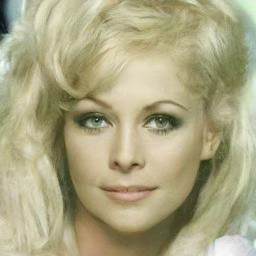
\includegraphics[width=\textwidth]{./figures/ddpm_steps1000_seed42_img_0}
        \caption{Styling from this image to apply}
    \end{subfigure}
    \begin{subfigure}[b]{0.25\textwidth}
        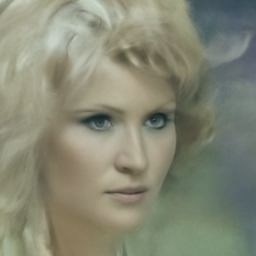
\includegraphics[width=\textwidth]{./figures/ddim_steps10_seed42_img_0}
        \caption{Original image without inpainting}
    \end{subfigure}
    \begin{subfigure}[b]{0.25\textwidth}
        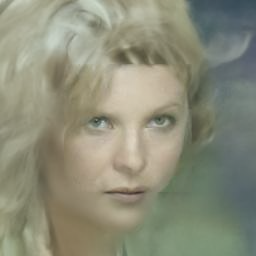
\includegraphics[width=\textwidth]{./figures/inpaint_steps1000_seed42_img_0}
        \caption{Image with inpainting from figure (a)}
    \end{subfigure}
    % \caption{Inpainting Output Images}
\end{figure}
\end{enumerate}